\subsection{Wagasci module}
The dimension of the each Wagasci module is 100cm $\times$ 100cm in the x and y directions
and 50cm along the beam direction.
Inside the Wagasci module, plastic scintillator bars are aligned as a 3D grid-like structure, shown in Fig. \ref{fig:3dgrid},
and spaces in the structure are filled with water for the water-in Wagasci module.

The total water mass serving as neutrino targets are $\sim$0.5 ton.
When neutrinos interact with hydrogen, oxygen or carbon, in water and scintillators,
charged particles are generated.
Neutrino interactions are identified by detecting tracks of charged particles through plastic scintillation bars.
Thanks to the 3 D grid-like structure of the scintillator bars, 
the Wagasci module has $4\pi$ angular acceptance for charged particles.
Furthermore, adopting a 5cm grid spacing, short tracks originated from protons and charged pions can be reconstructed
with high efficiency.
Thin plastic scintillator bars (thickness $\sim 0.3$cm) are used for the Wagasci module
to reduce  the mass ratio of scintillator bars to water,
because neutrino interactions in the scintillator bars are a background for the cross section measurements.
Scintillator bars whose dimensions are 2.5cm x 0.3cm x 100cm are used for the Wagasci module.
The total number of channels in one Wagasci module is 1280.

\begin{figure}[tbh]
\begin{center}
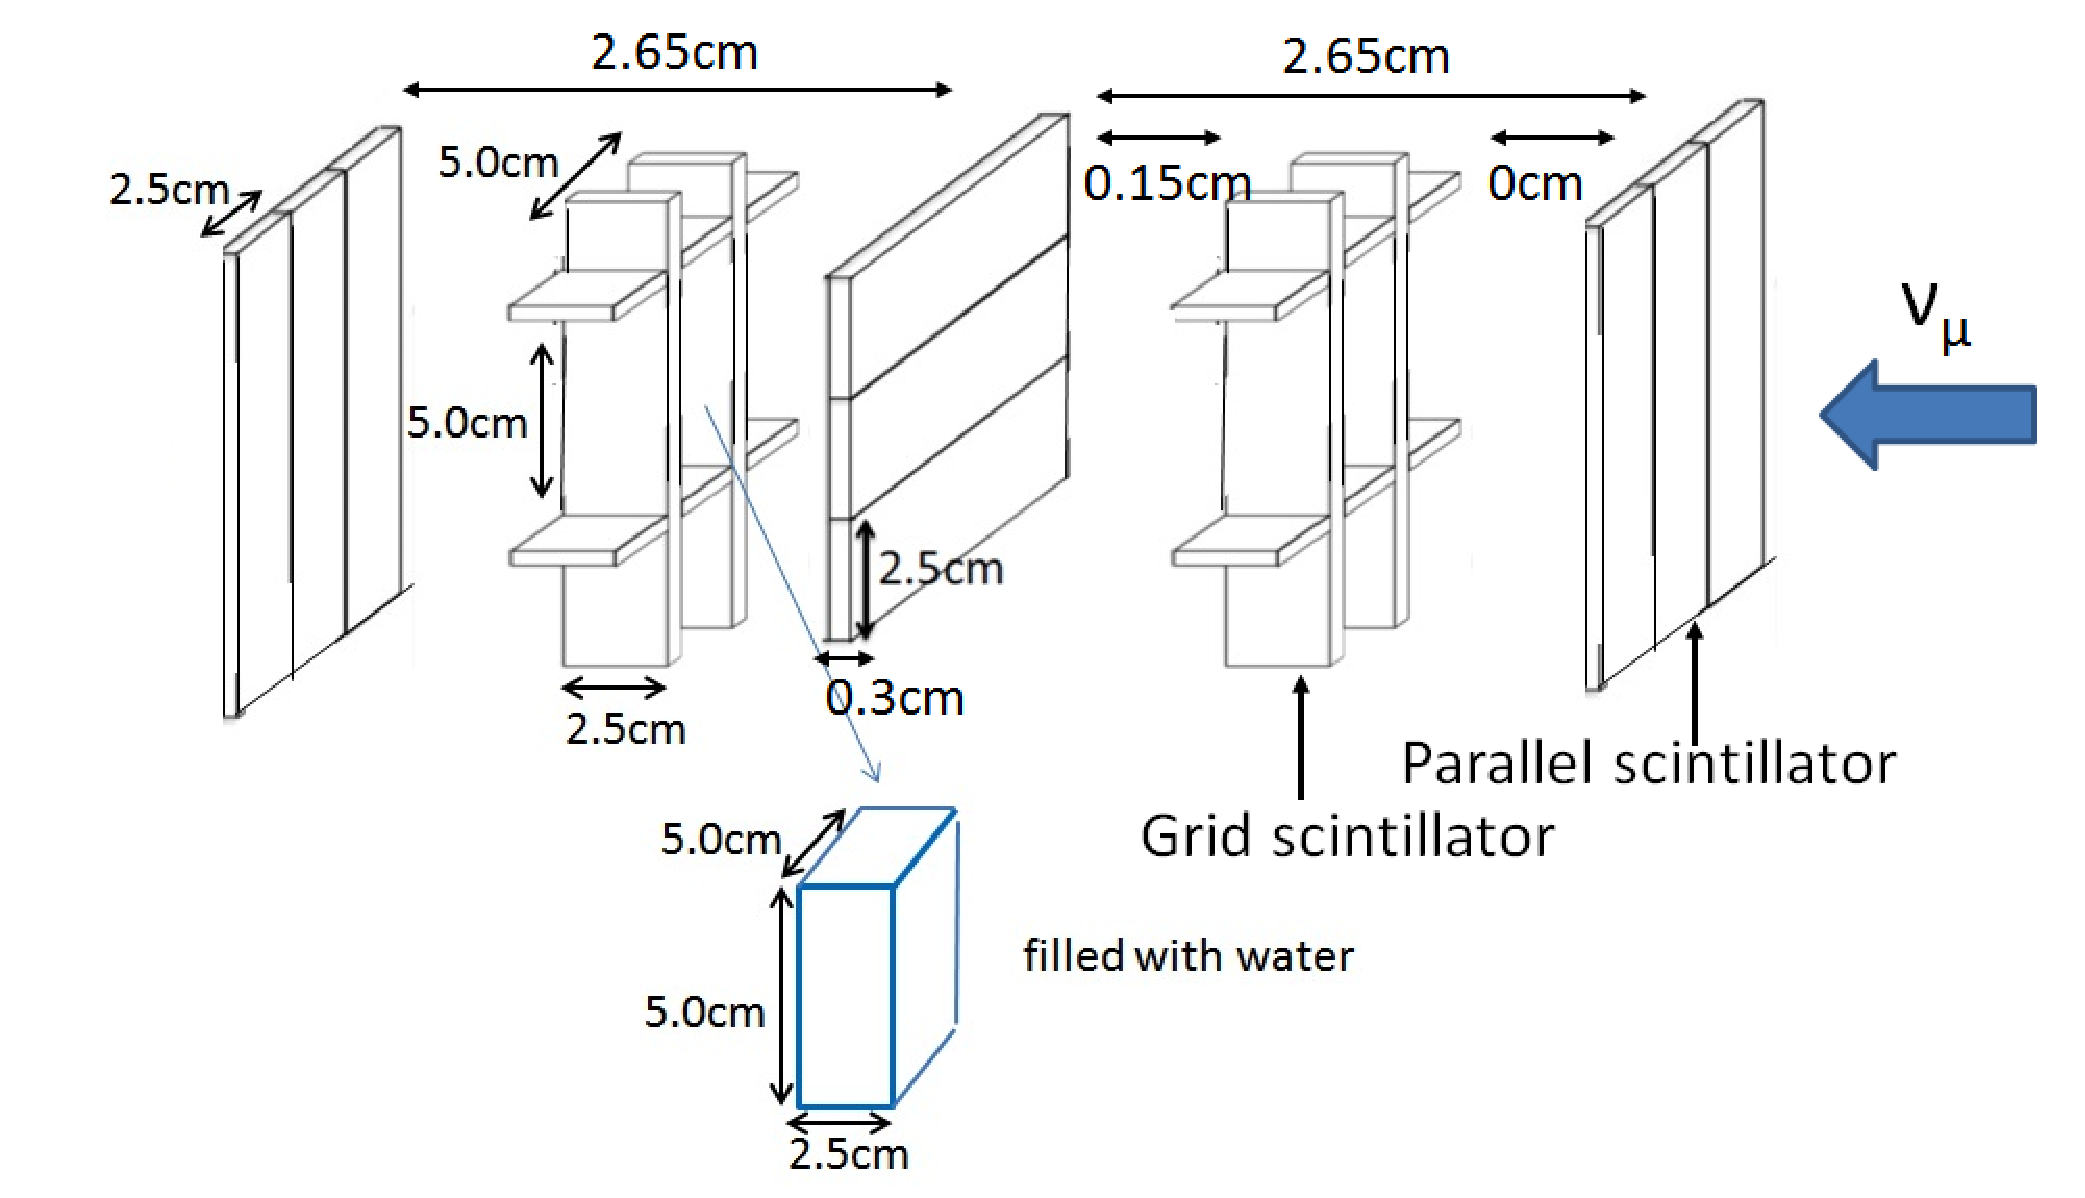
\includegraphics[width=1.0\linewidth]{fig/3d_grid_structure.pdf}
% 
\includegraphics[width=0.6\linewidth]{fig/tmp.pdf}
\end{center}
\caption{
Schematic view of 3D grid-like structure of plastic scintillator bars inside the central detector.
}
\label{fig:3dgrid}
\end{figure}

\begin{figure}[tbh]
\begin{center}
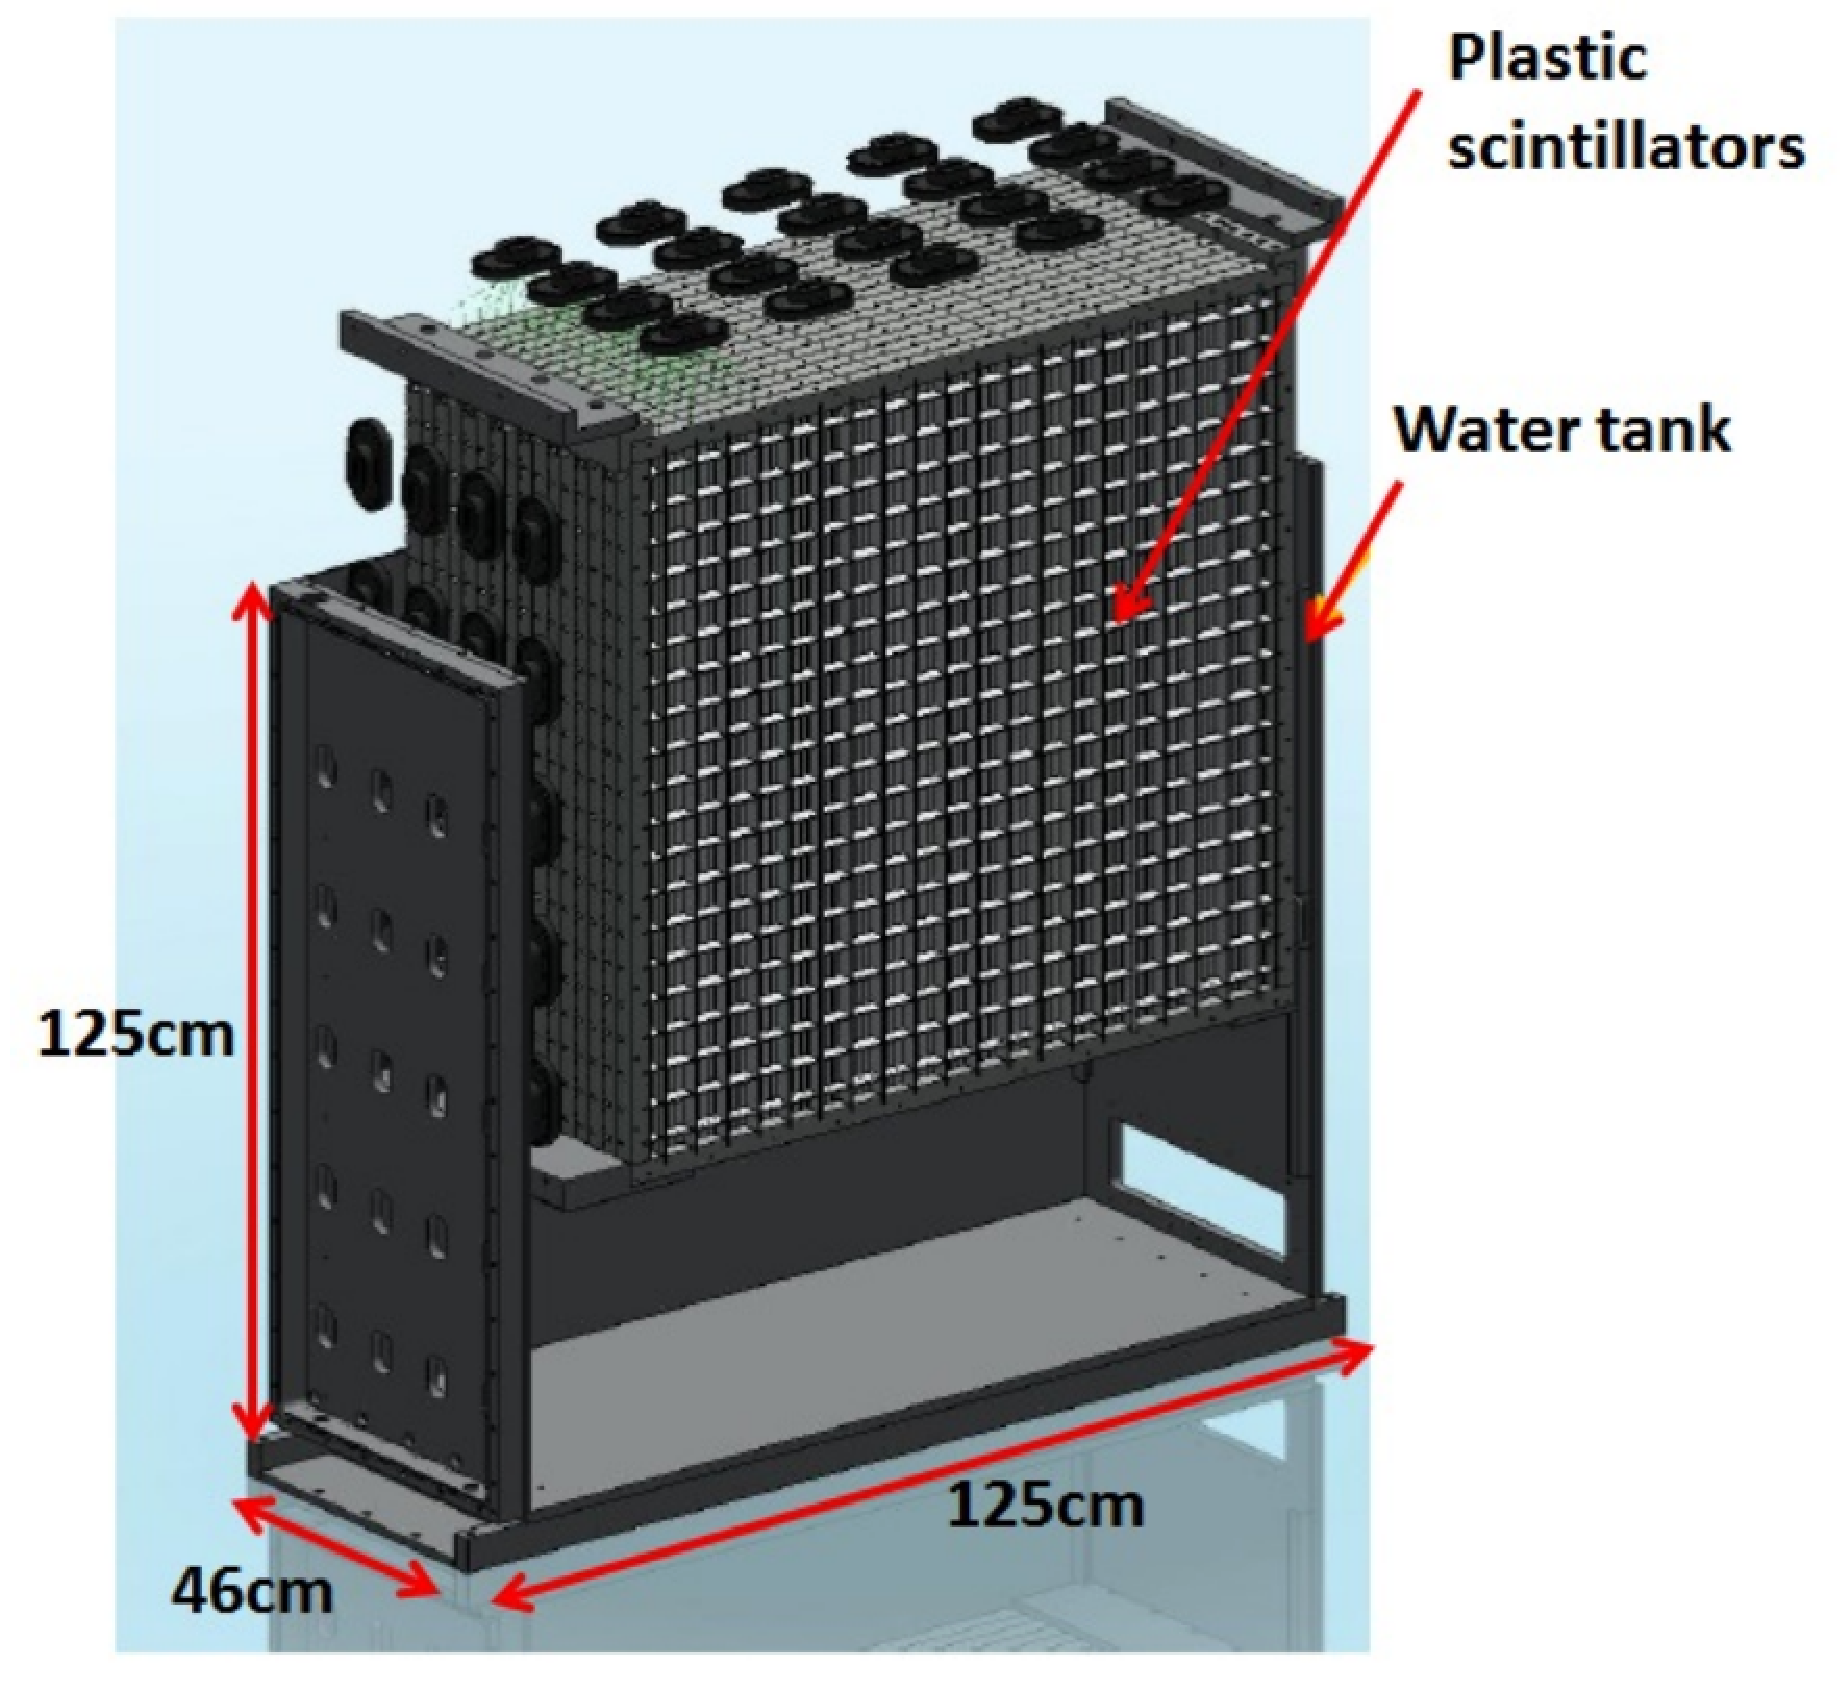
\includegraphics[width=0.6\linewidth]{fig/wagasci_mod.pdf}
% 
\includegraphics[width=0.6\linewidth]{fig/tmp.pdf}
\end{center}
\caption{
Schematic view of Wagasci module.
}
\label{fig:wagasci_mod}
\end{figure}
